\documentclass[red]{beamer}

\mode<presentation>
{
  \usetheme{Antibes}
  \usecolortheme{dolphin}
  \setbeamertemplate{footline}[frame number]
}

\usepackage[english]{babel}
\usepackage{subfigure}
\usepackage{xunicode}
\usepackage{xltxtra}
\usepackage{fontspec}
\usepackage{wrapfig}
\usepackage{subfigure}
\setmainfont{Ubuntu}

\title
{Master Information Evening \\
}

\author
{Jeroen Hofman}

\institute
{
 Department of Computational Science\\
 University of Amsterdam}

\pgfdeclareimage[height=0.8cm]{university-logo}{logo.png}
\logo{\pgfuseimage{university-logo}}

\begin{document}
\setbeamertemplate{navigation symbols}{}

\begin{frame}
  \titlepage
\end{frame}

\section{Introduction}

\begin{frame}{Background.}
  \begin{itemize}
  \item 
    BSc Physics \& Astronomy.
  \item
    One year at TU Delft (MSc Applied Physics).
  \item
    Currently master thesis at ING bank.
  \end{itemize}
\end{frame}

\begin{frame}{Personal experience with this programme.}
  Personal motivation:
  \begin{itemize}
  \item 
    Interdisciplinary subjects.
  \item
    More aimed at the world after graduation.
  \end{itemize}
  Experience:
  \begin{itemize}
  \item 
    Small classes.
  \item
    Wide variety of choices in courses.
  \item
    Project-based assignments, usually in groups.
  \item
    High motivation among students, high degree of independence.
  \item
    Good connection with the PhD-group and teachers/researchers.
  \end{itemize}
\end{frame}

\section{Courses}

\begin{frame}{Introduction in Computational Science.}
  \begin{itemize}
  \item 
    Correcting deficiencies.
  \item
    Introduction to certain types of models like dynamical systems.
  \end{itemize}
  \begin{figure}[H]
    \centering
    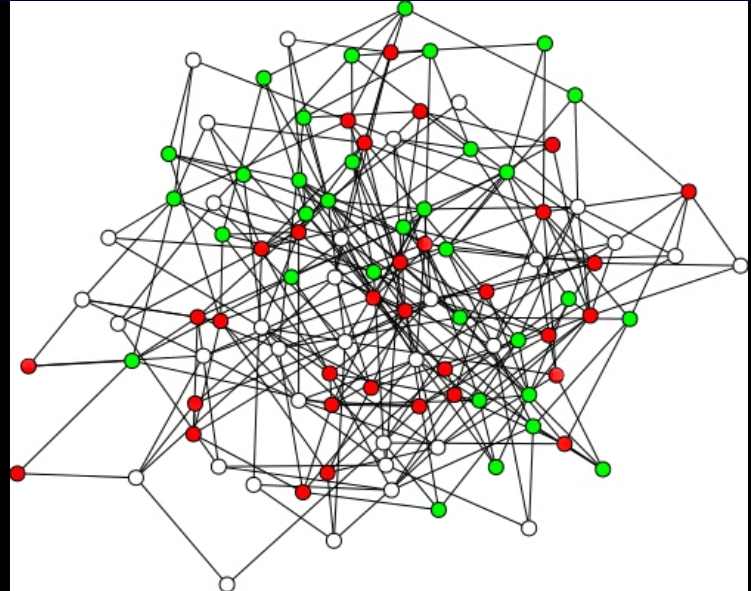
\includegraphics[width = 0.5\textwidth]{SIR.png}
    \caption{Disease spreading on a network.}
  \end{figure}
\end{frame}

\begin{frame}{Stochastic Simulation.}
  \begin{itemize}
  \item 
    How to use probability theory in modeling? $\rightarrow$ e.g. MC-simulations.
  \item
    Random number theory.
  \end{itemize}
  \begin{figure}[H]
    \centering
    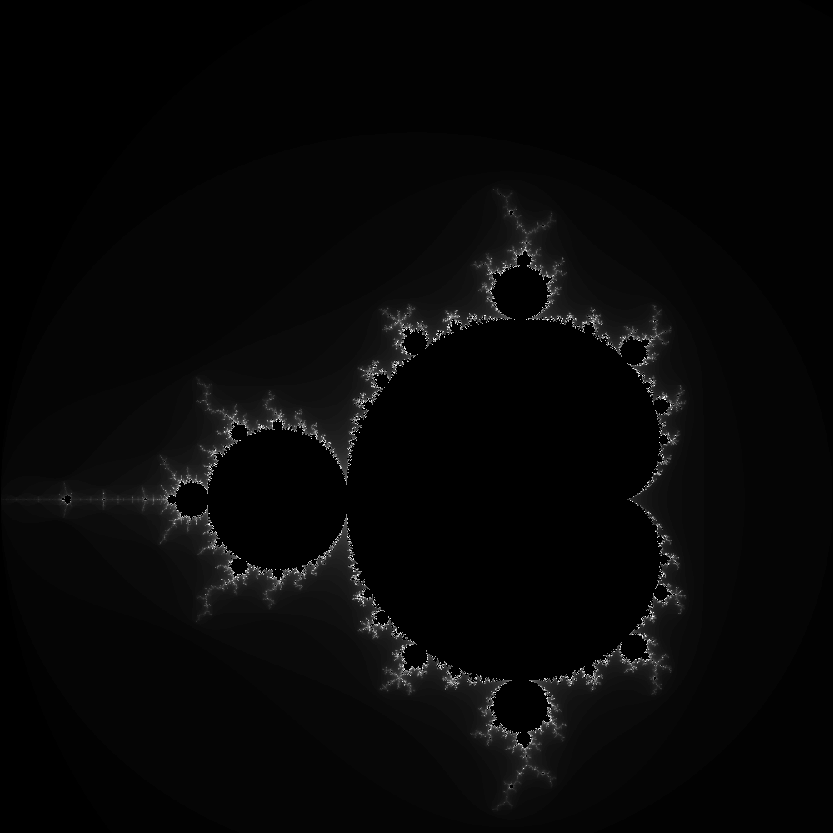
\includegraphics[width = 0.4\textwidth]{mandelbrot.pdf}
    \caption{Mandelbrot set.}
  \end{figure}
\end{frame}

\begin{frame}{Concurrent Programming.}
  \begin{itemize}
  \item 
    Learning about parallel paradigms and applications.
  \item
    Getting familiar with many paradigms (e.g. pThreads, MPI)
  \end{itemize}
  \begin{figure}[H]
    \centering
    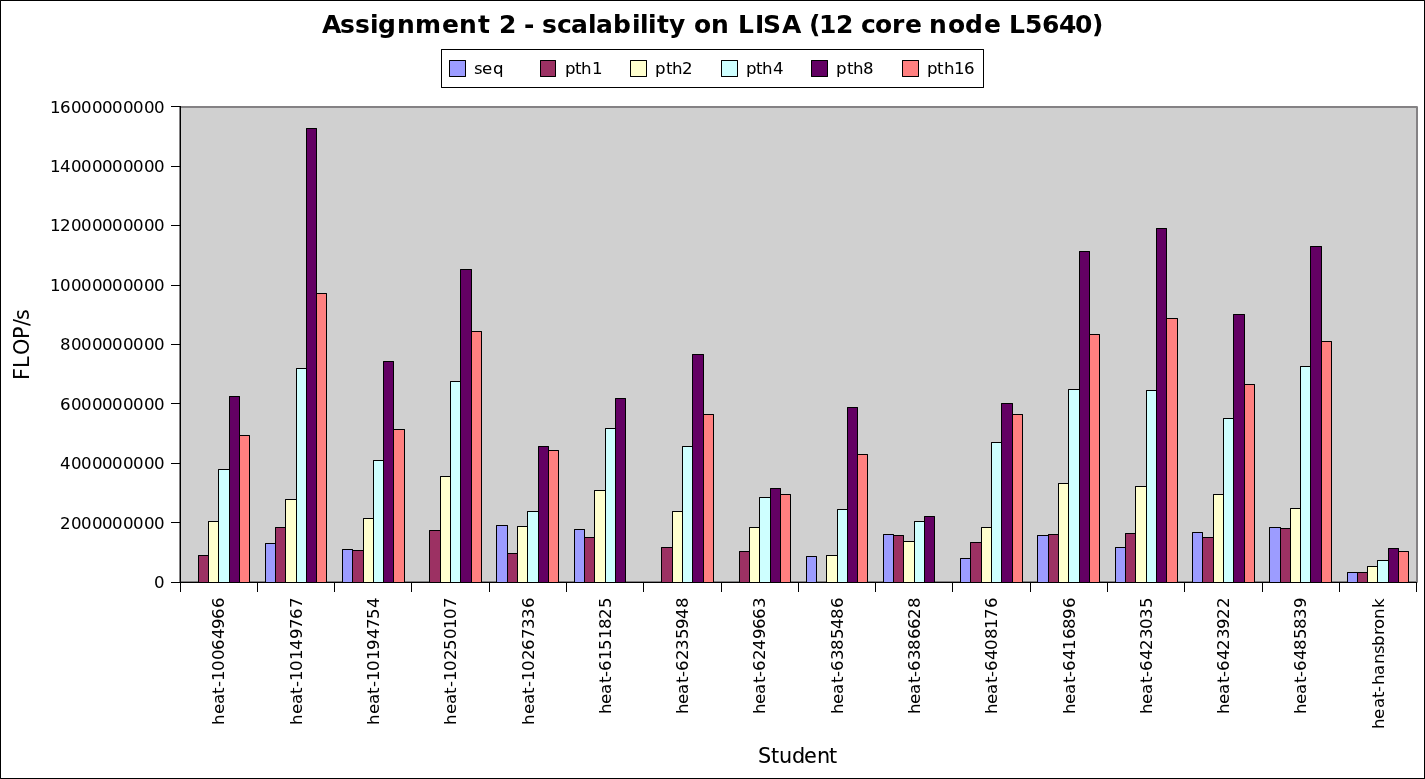
\includegraphics[width = 0.7\textwidth]{lisa.png}
    \caption{Competition on performance.}
  \end{figure}
\end{frame}

\begin{frame}{Computational Finance.}
  \begin{itemize}
  \item 
    Principles of quantitative finance.
  \item
    Derivation of important formulas for option pricing.
  \end{itemize}
  \begin{figure}[H]
    \centering
    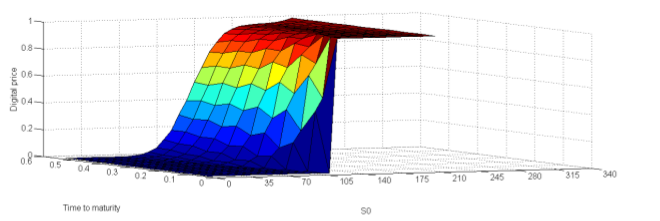
\includegraphics[width = 0.8\textwidth]{surface.png}
    \caption{Pricing surface of a digital option.}
  \end{figure}
\end{frame}

\begin{frame}{Complex System Simulation.}
  \begin{itemize}
  \item 
    Learning about complex (social) networks.
  \item
    Studying chaotic behavior.
  \end{itemize}
  \begin{figure}[H]
    \centering
    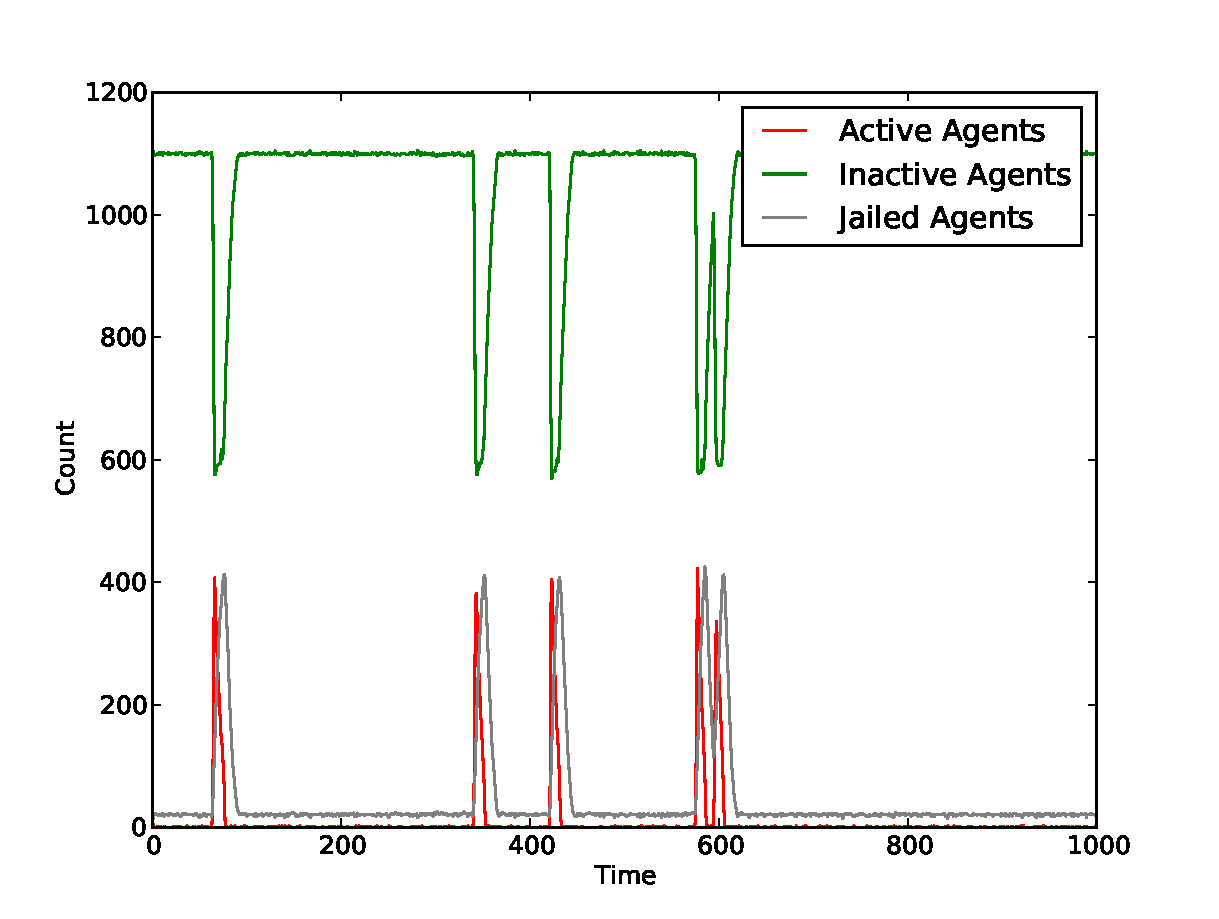
\includegraphics[width = 0.6\textwidth]{original_7.pdf}
    \caption{Rebel-cop interaction on a grid.}
  \end{figure}
\end{frame}

\begin{frame}{Scientific Visualization.}
  \begin{columns}[c]
    \column{.3\textwidth}
    \begin{itemize}
    \item 
      Studying about visualization methods used in scientific literature.
    \item
      Comparing visualization tools.
    \end{itemize}
    \column{0.7\textwidth}
    \begin{figure}[H]
      \centering
      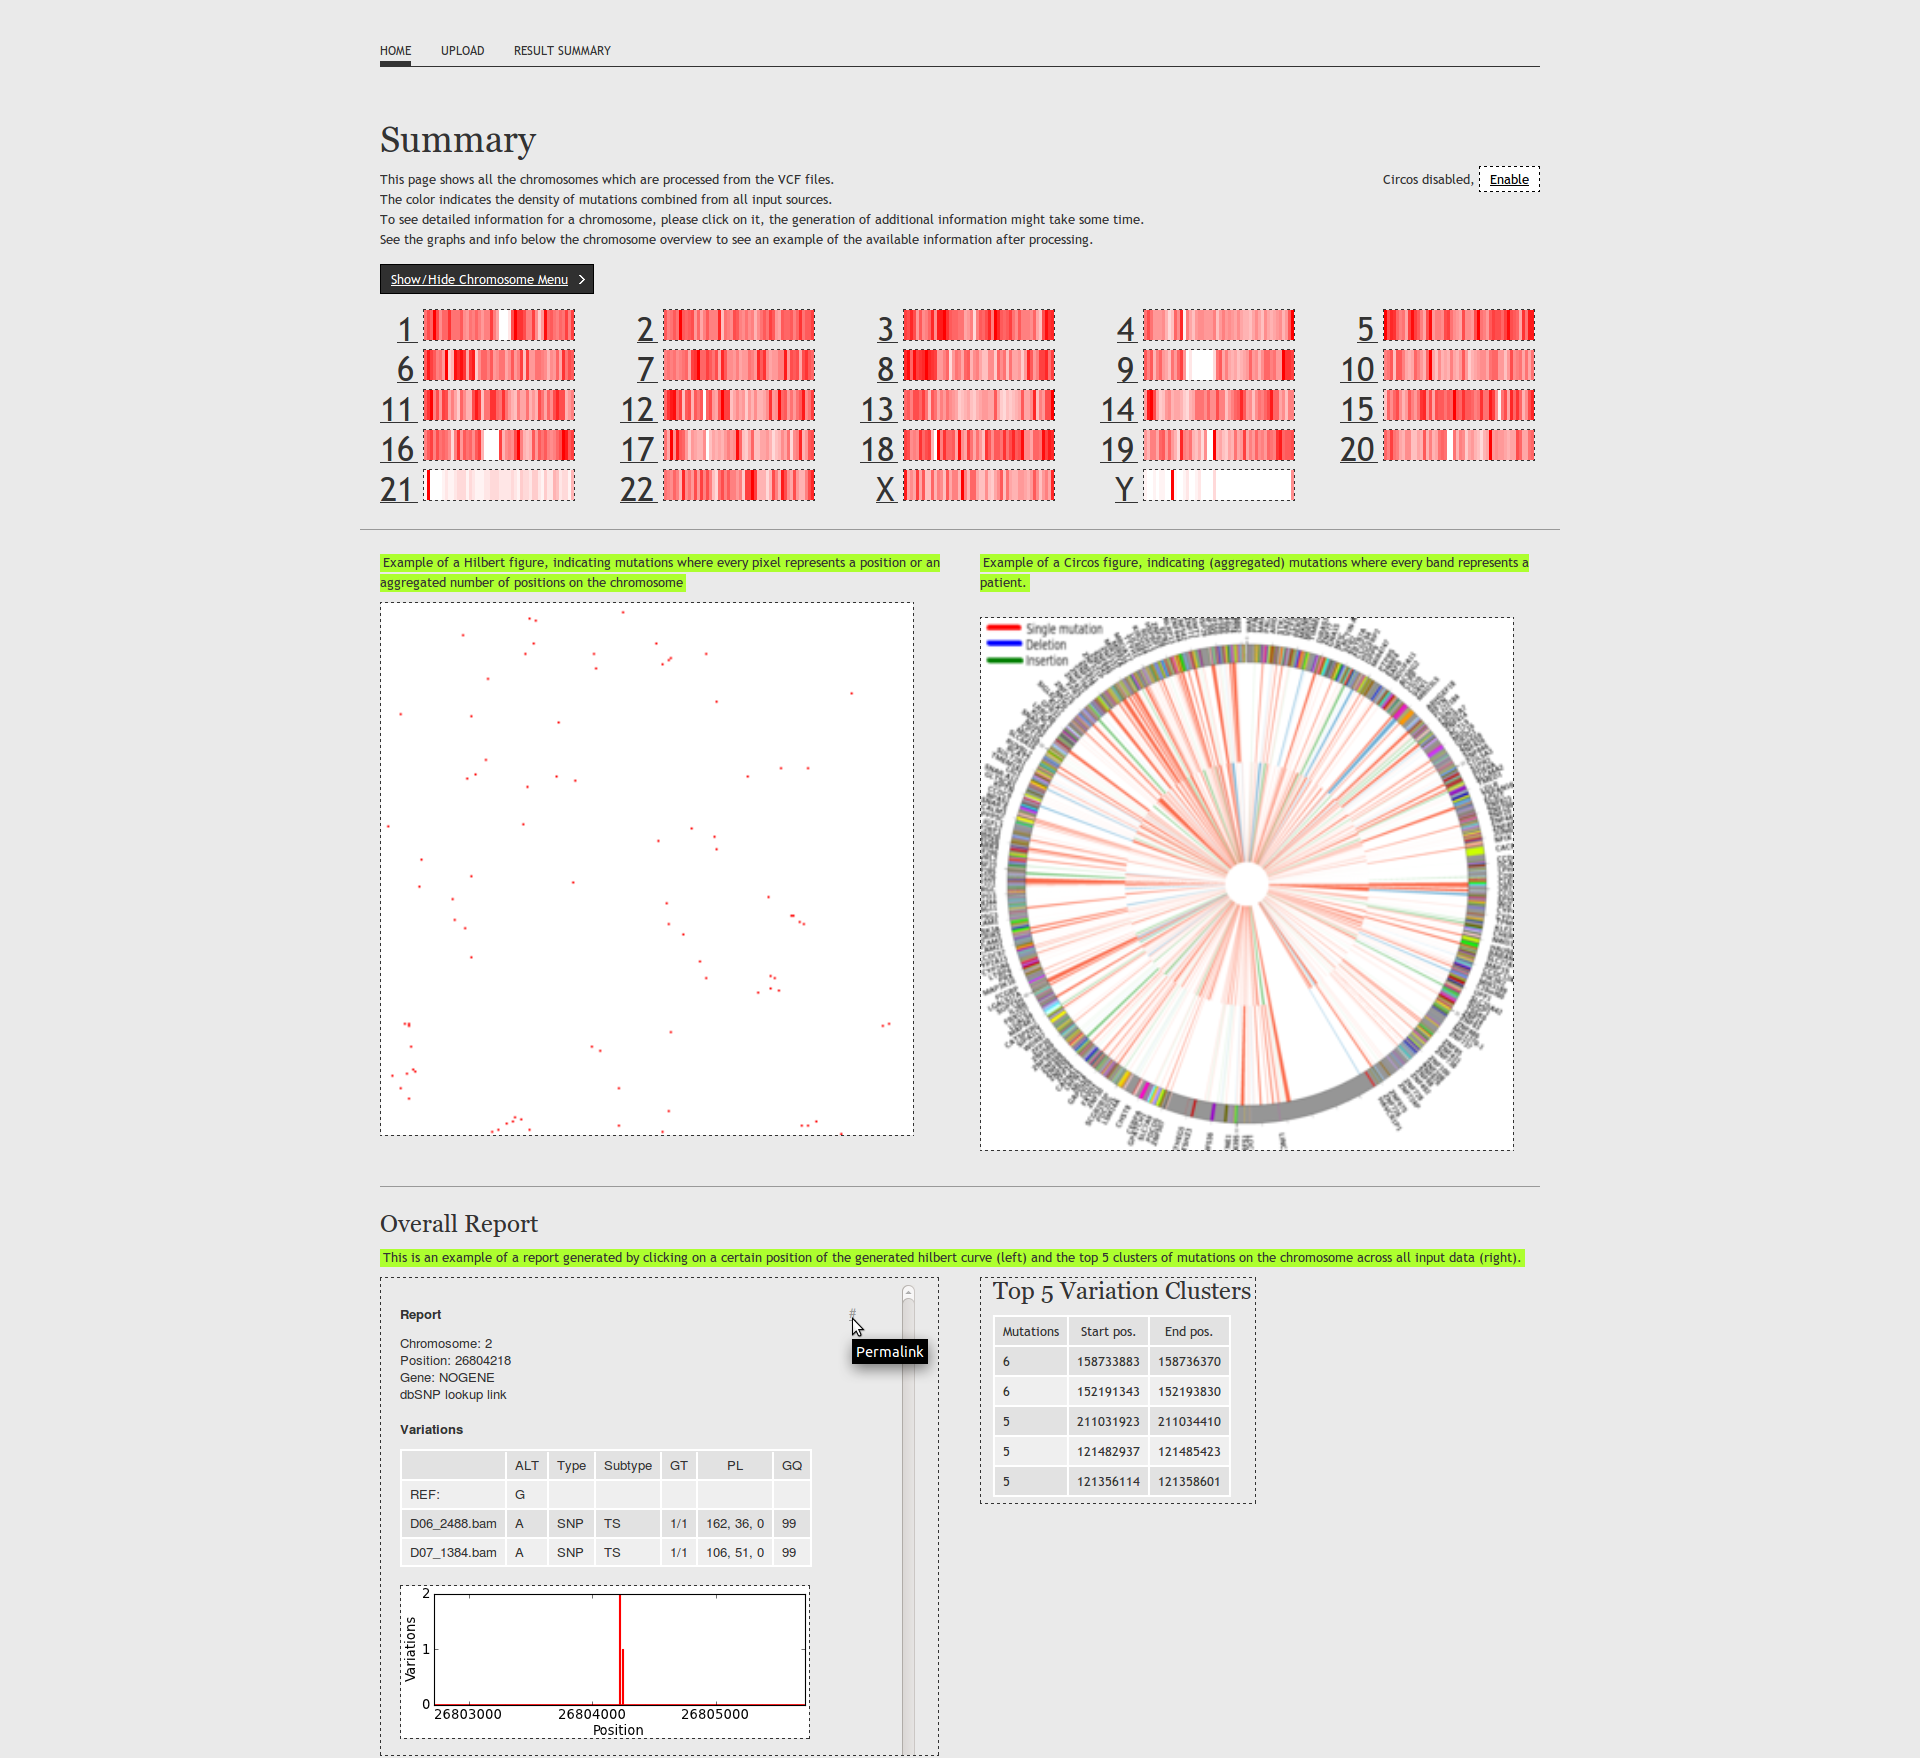
\includegraphics[width = 0.8\textwidth]{summarypage.png}
      \caption{DNAViewer: an interactive webpage for displaying mutation data.}
    \end{figure}
  \end{columns}
\end{frame}

\section{Master Thesis}

\begin{frame}{My Master Thesis.}
  \begin{itemize}
  \item 
    Currently doing my master project at ING.
  \item
    Topic: Valuation and hedging of Single Premium Variable Annuities (SPVA's).
  \item
    Computational finance uses many principles from physics, e.g.:\\
    \begin{equation*}
      \frac{\partial V}{\partial t} + \frac{1}{2}\sigma^2 S^2 \frac{\partial^2 V}{\partial S^2} + rS\frac{\partial V}{\partial S} - rV = 0
    \end{equation*}
  \end{itemize}
\end{frame}

\begin{frame}{Others.}
  \begin{itemize}
  \item 
    Iona Niculescu, Modeling cells in blood vessel systems, Comp. Science UvA.
  \item
    Louis Dijkstra: Dynamic social-economic networks, University of St. Petersburg.
  \item
    Cong Chen: Potts-model research, CWI.
  \item
    Alex Thiakos: Insurance-related development of pricing methods, ING.
  \item
    Lotte Huisman: Multi-scale modeling of calcification in scleractinian corals, Comp. Science UvA/James Cook University.
  \item
    Amir Masoud Abdol: Multi-objective optimization for modeling developmental gene regulatory networks, Comp. Science UvA/Centre for Regulatory Genomics Barcelona.
  \end{itemize}
\end{frame}

\section{The End}

\begin{frame}
  \begin{center}
    \vspace{20pt}
    \huge{Thank you for your attention!}\\
    \vspace{15pt}
    \Large{Questions?}
  \end{center}
\end{frame}

\end{document}